\documentclass[12pt,spanish]{article}
\usepackage[spanish]{babel}
\usepackage{graphicx}
\usepackage{color}
\usepackage{xcolor}
\usepackage{colortbl}
\usepackage{multirow}
\usepackage{amsmath}
\usepackage{subcaption}
\usepackage{adjustbox}
\usepackage{multirow}
\usepackage[hidelinks]{hyperref}
\usepackage{caption}
\usepackage{amsthm}
\usepackage{multicol}
\usepackage[outputdir=build]{minted}
\usepackage{float}
\usepackage{titling}
\usepackage{soul}
\usepackage{listings}
\usepackage{array}
\graphicspath{ {./img/} {../../LaTeX/img/}}
\selectlanguage{spanish}
\usepackage[utf8]{inputenc}
\usepackage{graphicx}
\usepackage[a4paper,left=3cm,right=2cm,top=2.5cm,bottom=2.5cm]{geometry}
\newtheorem{definition}{Definición}



\title{Fundamentos de Bases de Datos}
\setlength{\droptitle}{10em}
\author{Carlos Sánchez Páez}

\makeindex
\begin{document}


\begin{titlepage}

\newlength{\centeroffset}
\setlength{\centeroffset}{-0.5\oddsidemargin}
\addtolength{\centeroffset}{0.5\evensidemargin}
\thispagestyle{empty}

\noindent\hspace*{\centeroffset}
\begin{minipage}{\textwidth}

\centering

\includegraphics[width=0.9\textwidth]{logo_ugr.jpg}\\[1.4cm]

\textsc{ \Large Fundamentos de Bases de Datos\\[0.2cm]}
\textsc{GRADO EN INGENIERÍA INFORMÁTICA}\\[1cm]

{\Huge\bfseries Resumen del temario\\}
\end{minipage}

\vspace{1.5cm}
\noindent\hspace*{\centeroffset}
\begin{minipage}{\textwidth}
\centering

\textbf{Autor}\\ {Carlos Sánchez Páez}\\[2.5ex]

\includegraphics[width=0.3\textwidth]{etsiit_logo.png}\\[0.1cm]
\vspace{1.5cm}

\includegraphics[width=0.5\textwidth]{decsai.jpg}\\[0.1cm]
\vspace{1cm}
\textsc{Escuela Técnica Superior de Ingenierías Informática y de Telecomunicación}\\
\vspace{1cm}
\textsc{Curso 2017-2018}
\end{minipage}
\end{titlepage}
\thispagestyle{empty}
\newpage
\tableofcontents{}
\newpage
\listoffigures
\thispagestyle{empty}
\newpage

\section{Tema 1. Introducción y definiciones iniciales.}

\subsection{Concepto intuitivo de bases de datos}

Prácticamente todas las empresas necesitan aplicacioens que gestionen información a la que se accederá desde distintos puntos. Si estos datos pertenecen a las aplicaciones, hay tres problemas principales:
\begin{itemize}
	\item \textbf{Redundancia}. La información se repite en varios sitios a la vez.
	\item \textbf{Inconsistencia}. ¿Cuáles son los datos más actualizados?
	\item \textbf{No hay reutilización}. 
\end{itemize}

Si utilizamos ficheros, podemos hacer que la información sea compartida, sin embargo:
\begin{itemize}
	\item Tenemos que mantener una estructura determinada.
	\item Debemos proteger los archivos de ciertos usuarios.
	\item Debemos permitir el acceso con distintos lenguajes y sistemas operativos.
\end{itemize}

\begin{figure}[H]
\centering
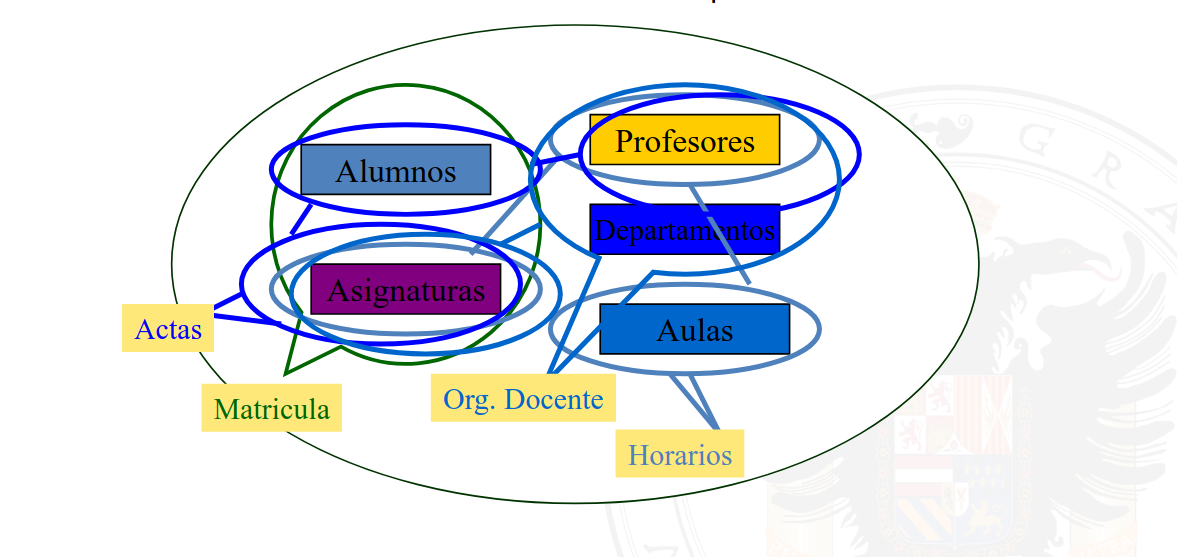
\includegraphics[scale=0.25]{redundancia_archivos.png}
\caption{Acceso a archivos desde diferentes aplicaciones.}
\end{figure}

Por tanto, la solución final es \textbf{una base de datos}.

\begin{definition}[Base de datos]
Una \emph{base de datos} es un conjunto de datos comunes a un \textit{proyecto} almacenados sin redundancia para ser útiles a distintas aplicaciones.
\end{definition}

\begin{definition}[Sistema gestor de bases de datos]
Un \emph{sistema gestor de bases de datos (SGBD)} es un conjunto de elementos software con la capacidad para definir, mantener y utilizar una base de datos.
\end{definition}

Un SGBD debe permitir:
\begin{itemize}
\item \textbf{Definir} estructuras de almacenamiento.
\item \textbf{Acceder} a los datos de forma eficiente y segura.
\item Organizar la \textbf{actualización} de los datos y el \textbf{acceso} multiusuario.
\item etc.
\end{itemize}

Resumiendo, una base de datos es un fondo común de información almacenada en una computadora para que cualquier persona o programa autorizado pueda acceder a ella, independientemente del lugar de procedencia  y el uso que haga de la misma.\\

Con un SGBD podemos gestionar datos y una estructura de datos de forma transparente (sin tener que programar un código específico):
	\begin{itemize}
		\item \textbf{Insertar} datos.
		\item \textbf{Modificar} datos existentes.
		\item \textbf{Borrar} datos existentes.
		\item \textbf{Obtener} datos previamente insertados.
	\end{itemize}
Normalmente estas operaciones se denominan CRUD (\textbf{C}reate, \textbf{R}ead, \textbf{U}pdate y \textbf{D}elete).


\subsection{Bases de datos y sistemas de gestión de bases de datos.}

Una base de datos involucra:

\begin{itemize}
	\item \textbf{Datos}
		\begin{itemize}
			\item Integrados (sin redundancia).
			\item Compartidos (útiles a varias aplicaciones).
		\end{itemize}
		\item \textbf{Hardware}
			\begin{itemize}
				\item Base de datos normal.
				\item Base de datos distribuida.
			\end{itemize}
		\item Software \textbf{DBMS} (DataBase Management System). SOn programas par describir las estructuras y gestionar la información de la base de datos.
		\item \textbf{Usuarios}
			\begin{itemize}
				\item Usuario final.
				\item Programador de aplicaciones.
				\item Administrador (DBA ó DBM).
			\end{itemize}
\end{itemize}

\begin{definition}[Dato operativo]
Un \textbf{dato operativo} es una pieza de información básica que necesita una empresa, proyecto o aplicación para su funcionamiento.
\end{definition}

Un dato operativo puede ser:
\begin{itemize}
	\item \textbf{Ítem básico}. Elementos acerca de los que se puede pedir información (sustantivos).
	\item \textbf{Atributos}. Características de los ítems básicos (adjetivos o propiedades de los ítems).
	\item \textbf{Relaciones}. Conexiones lógicas entre ítems.
\end{itemize}

Cuando se determinan y se clasifican así todos los datos operativos obtenemos el \emph{esquema lógico} de la base de datos.\\

En el día a día, usaremos el término \textbf{campo} para referirnos a la representación de un dato o atributo en la base de datos.

Ejemplos de dato operativo:

\begin{itemize}
	\item \textbf{Ítem básico}. Estudiante, asignatura, paciente, etc.
	\item \textbf{Atributos}. Nombre, apellidos, relación, etc.
	\item \textbf{Relaciones}. Estudiante \textbf{está matriculado en} asignatura, profesor \textbf{imparte} asignatura, etc.
\end{itemize}

\begin{figure}[H]
\centering
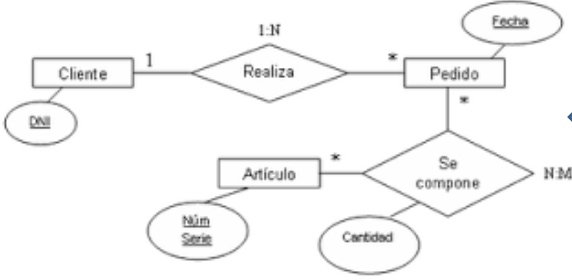
\includegraphics[scale=0.5]{ejemplo_er.png}
\caption{Ejemplo de diagrama entidad-relación.}
\end{figure}

\subsection{Concepto de independencia}

\begin{definition}[Independencia]
	Los datos se organizan independientemente de las aplicaciones que los vayan a usar de los archivos en los que vayan a almacenarse.
\end{definition}

\begin{definition}[Independencia física]
	El diseño lógico de la base de datos debe ser independiente del almacenamiento físico de los datos.
\end{definition}

Ésto permite:

\begin{itemize}
	\item Realizar cambios en la estructura física sin alterar la lógica de la aplicación (representación de campos, organización en registros, mecanismos de acceso, etc.)
	\item Liberar a las aplicaciones de la misión de gestionara aspectos relativos al almacenamiento.
\end{itemize}

\begin{definition}[Independencia lógica]
	Cada aplicación debe poder organizar lso datos según sus propios esquemas y acceder a los datos que le son necesarios y le conciernen (vistas de usuario).
\end{definition}

La independecia lógica provoca varias mejoras:
\begin{itemize}
	\item Aumento de seguridad y fiabilidad.
	\item Menos problemas para las aplicaciones.
	\item Posibilidad de cambios en los esquemas por parte de desarrolladores de aplicaciones y administradores.
\end{itemize}

El \textbf{esquema lógico general} permite organizar la información global de toda la organización para optimizar accesos, evitar redundancia, etc.\\

La \textbf{vista de usuario} permite dar permiso a los programadores de las aplicaciones para acceder a los datos que pueden ver del esquema general, ocultando los datos a los que no se debe tener acceso.\\

\subsection{Objetivos de un SGBD}

Los objetivos de un sistema de gestión de bases de datos son:

\begin{itemize}
	\item \textbf{Independencia de los datos}.
	\item \textbf{Utilización y diseño orientados al usuario}. Los datos y aplicaciones deben ser accesibles a los usuarios de la forma más amigable posible.
	\item \textbf{Centralización}. Los datos deben gestionarse de forma centralizada e independiente de las aplicaciones.
	\item \textbf{Eliminación de redundancia}. Los datos no pueden estar duplicados y se deben gestionar los accesos concurrentes.
	\item \textbf{Consistencia}. Los datos deben ser consistentes (sin fallos lógicos) y se deben implementar mecanismos para mantener la integridad.
	\item \textbf{Fiabilidad}. Los datos deben estar protegidos contra fallos, para lo que son necesarios mecanismos de mantenimiento, recuperación y realizamiento de transacciones.
	\item \textbf{Seguridad}. No todos los datos deben ser accesibles a todos los usuarios.
\end{itemize}

Hay varios tipos de usuario en una base de datos:

\begin{itemize}
	\item \textbf{Usuario final}. Debe poder acceder a los datos.
	\item \textbf{Programador de aplicaciones}. Debe eliminar problemas de diseño, depuración y mantenimiento.
	\item \textbf{Administrador}. Su cometido surge con la aparición de la base de datos.
\end{itemize}

En cuanto al sistema:

\begin{itemize}
	\item Control \textbf{centralizado}.
	\item Criterios de \textbf{uniformización}.
	\item Generación de \textbf{nuevas aplicaciones}.
	\item \textbf{Equilibrio} entre requierimientos conflictivos.
\end{itemize}

\section{Tema 2. Arquitectura de un sistema gestor de bases de datos.}















\end{document}